 \chapter{Samples based CdTe}
\label{chap:appendix2}
\textit{In this annex the results obtained from the modifications made on HgCdTe and CdTe samples are discussed. Mechanical modifications on the surface and silver evaporations were performed with the objective of understanding the behavior of a metal on a semiconductor. The idea of modifying the surfaces by evaporating was proposed, due to the intention of understanding in a fundamental way the novel materials known as topological insulators and given the particular phenomena that were presented in the HgCdTe quantum wells under considerations that will be addressed in this annex, the proposal is to study CdTe surfaces with Ag evaporations with the help of the e-beam coupled in the vacuum chamber.}
\vfill
\minitoc
\newpage

\allowdisplaybreaks
\section{Samples Descriptions}
\vspace{-1cm}

\newcolumntype{C}{>{\centering\arraybackslash}p{80mm}}% a centered fixed-width-column
\begin{table}[H]
	\centering
	\begin{tabular}{lC}
		\hline
		\hline
		&  Description\\
		\hline
		Sample 01 & CdTe \\
		Sample 02 & HgCdTe\\
		Sample 03 & HgCdTe\\
		Sample 04 & HgCdTe con superficie tallada \\
		Sample 05 & HgCdTe con superficie evaporada\\
		Sample 06 & CdZnTe\\
		\hline
		\hline
	\end{tabular}
	\caption{Samples studied from the $CdTe$ family}
	\label{tab:CH 3 Section 3.1 Photodectors materials}
\end{table}

\begin{figure}[htp] 
	\centering
	
	\subfloat[data a]{%
	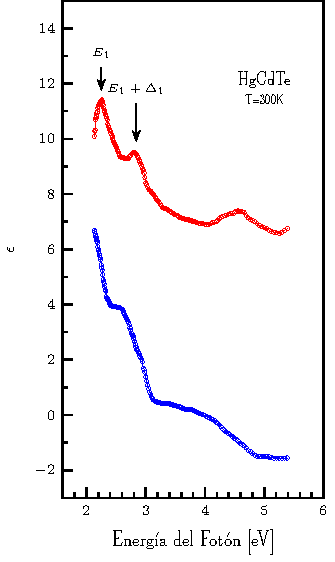
\includegraphics[width=0.4\textwidth]{FIGURES/Anexo-CdTe/fd-hgcdte.pdf}%
	\label{fig:a}%
	}
	\subfloat[data b]{%
	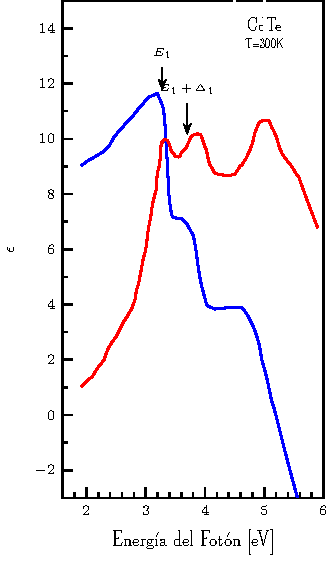
\includegraphics[width=0.4\textwidth]{FIGURES/Anexo-CdTe/fd-CdTe.pdf}%
	\label{fig:b}%
	}
	
	\caption{all the data}
\end{figure}

\begin{figure}[htp] 
	\centering
	
	\subfloat[data a]{%
	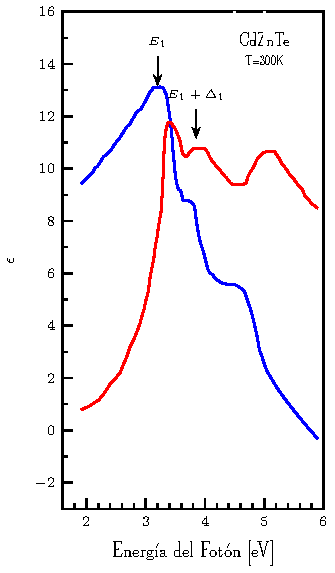
\includegraphics[width=0.4\textwidth]{FIGURES/Anexo-CdTe/fd-CdZnTe.pdf}%
	\label{fig:a}%
	}
	\subfloat[data b]{%
	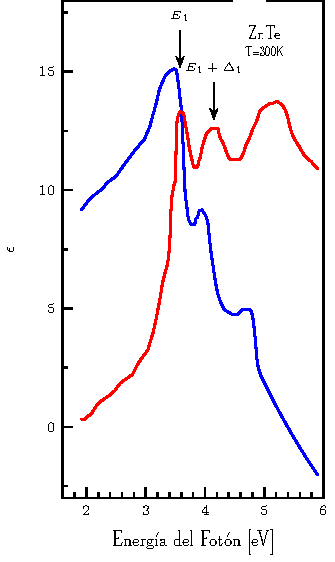
\includegraphics[width=0.4\textwidth]{FIGURES/Anexo-CdTe/fd-ZnTe.pdf}%
	\label{fig:b}%
	}
	
	\caption{all the data}
\end{figure}

\subsection{CdTe}

\subsection{CdZn}

\subsection{ZnTe}

\subsection{CdZnTe}
\section{Results an Conclusions}